\section{The spin-zero superfluid of the spinor charges}
\label{sec:superfluid}

\subsection{The field content from the bi-octonion product}

Write a spinor charge $\mathbf b\,\mathbf e_4$ through the $2\times2$ matrix $M_{\rm LL}(\mathbf b)$ of
Sec.~\ref{sec:bioct}. The Lorentz derivation~(\ref{eq:dlor}) multiplies $\mathbf b$ by $-\mathbf u$ from
the right, which acts within each row of $M_{\rm LL}(\mathbf b)$; the isospin derivation~(\ref{eq:diso})
multiplies from the left, which mixes the two rows. Define the $2\times2$ matrix
\begin{equation}
\psi'_{\rm LL}=\mathsf E_{\rm LL}^{-1}M_{\rm LL}(\mathbf b)^T,\qquad \mathsf E_{\rm LL}=i\sigma^{\rm LL}_2 .
\label{eq:psiprime}
\end{equation}
Its first column (isospin up) and its second column (isospin down) are Weyl spinors: on each column the
Lorentz derivations act as $D_{\rm LL}(J^j_{\rm LL})=-\tfrac{i}{2}\sigma^{\rm LL}_j$ and $D_{\rm
LL}(K^j_{\rm LL})=+\tfrac12\sigma^{\rm LL}_j$, and the isospin generators $T^\iota_{\rm LL}$ act on the
column index as $\tfrac12\tau^{\rm LL}_\iota$ (check S-0; the step uses $\mathsf E_{\rm
LL}^{-1}(\sigma^{\rm LL}_j)^T\mathsf E_{\rm LL}=-\sigma^{\rm LL}_j$).

In the chiral basis the Dirac matrices are $\gamma^0_{\rm LL}=\begin{pmatrix}0&\sigma^{\rm
LL}_0\\\sigma^{\rm LL}_0&0\end{pmatrix}$, $\gamma^j_{\rm LL}=\begin{pmatrix}0&\sigma^{\rm
LL}_j\\-\sigma^{\rm LL}_j&0\end{pmatrix}$, with the chirality matrix $\gamma^{\rm ch}_{\rm LL}=i\gamma^0_{\rm
LL}\gamma^1_{\rm LL}\gamma^2_{\rm LL}\gamma^3_{\rm LL}=\mathrm{diag}(-1,-1,1,1)$ and the charge-conjugation
matrix $C_{\rm LL}=i\gamma^2_{\rm LL}\gamma^0_{\rm LL}$~\cite{PeskinSchroeder1995}. The spinor charges, on
which $D_{\rm LL}(K^j_{\rm LL})=+\tfrac12\sigma^{\rm LL}_j$, are the lower block ($\gamma^{\rm ch}_{\rm
LL}=+1$); the complex-conjugate super-loop, on which the boosts act with the opposite sign, supplies the
upper block. The Dirac matrices intertwine these spinor generators with the action of the loop's
conjugations on $\mathbb R^{1,3}_{\rm LL}$: for each of the six generators, $[\gamma^p_{\rm LL},\cdot\,]$
reproduces the vector action $\mathcal V_{\rm LL}$ (all 24 relations of S-0). The field of the
spinor charges is therefore a \emph{Dirac isodoublet} $\Psi_{\rm LL}$ with 8 components (Dirac $\otimes$
isospin), with electric charges $Q_{\rm LL}=\pm\tfrac12$. Its components have spinor number $-1$, so, by
the spin-statistics theorem of relativistic quantum field theory, $\Psi_{\rm LL}$ is a fermion field: its
components anticommute.

The Hamiltonian is that of free Dirac particles of mass $m_{\rm LL}$ at the chemical potential $\mu_{\rm
LL}$, with an attractive contact interaction in the spin-zero channels of Theorem SF1 below,
\begin{equation}
\mathcal H^{\rm sf}_{\rm LL}=\sum_{\vec q_{\rm LL}}\Psi^\dagger_{\rm LL}(\mathsf h_{\rm LL}-\mu_{\rm LL})\Psi_{\rm LL}-\tfrac14G_{\rm LL}\sum_\iota(\Pi^\iota_{\rm LL})^\dagger\Pi^\iota_{\rm LL},
\label{eq:ham}
\end{equation}
with $\mathsf h_{\rm LL}(\vec q_{\rm LL})=\sum_j\alpha^j_{\rm LL}q^j_{\rm LL}+\beta_{\rm LL}m_{\rm LL}$
(times $\sigma^{\rm LL}_0$ on the isospin index), $\alpha^j_{\rm LL}=\gamma^0_{\rm LL}\gamma^j_{\rm LL}$,
$\beta_{\rm LL}=\gamma^0_{\rm LL}$, and the pair operators $\Pi^\iota_{\rm LL}=\sum_{\vec q_{\rm
LL}}\Psi_{\rm LL}(\vec q_{\rm LL})^T\mathsf K^\iota_{\rm LL}\Psi_{\rm LL}(-\vec q_{\rm LL})$, which annihilate
two spinor charges of opposite momenta. Momentum sums run over $q_{\rm LL}<\Lambda_{\rm LL}$.

\subsection{The spin-zero channels}

\noindent\emph{Theorem SF1.} The antisymmetric $8\times8$ matrices $\mathsf K$ for which the pair
$\Psi^T_{\rm LL}\mathsf K\Psi_{\rm LL}$ is Lorentz invariant form a complex space of dimension 6, spanned by
\begin{equation}
\mathsf K^\iota_{\rm LL}=C_{\rm LL}\gamma^{\rm ch}_{\rm LL}\otimes\mathsf E_{\rm LL}\tau^{\rm LL}_\iota,\quad \mathsf K'^\iota_{\rm LL}=C_{\rm LL}\otimes\mathsf E_{\rm LL}\tau^{\rm LL}_\iota
\label{eq:channels}
\end{equation}
($\iota=1,2,3$; scalar $0^+$ and pseudoscalar $0^-$). Every spin-zero s-wave pair of spinor charges is
an isospin \emph{triplet}, with the electric charges $+1$, $0$, $-1$.

\noindent\emph{Proof.} The Lorentz-invariant bilinear forms of a Dirac spinor are those of
$(\tfrac12,0)\otimes(\tfrac12,0)$ and $(0,\tfrac12)\otimes(0,\tfrac12)$, one each, spanned by $C_{\rm
LL}=\mathrm{diag}(\mathsf E_{\rm LL},-\mathsf E_{\rm LL})$ and $C_{\rm LL}\gamma^{\rm ch}_{\rm
LL}=-\mathrm{diag}(\mathsf E_{\rm LL},\mathsf E_{\rm LL})$; both are antisymmetric. For anticommuting
components only the antisymmetric part of $\mathsf K$ contributes, so the isospin factor must be
symmetric. The symmetric $2\times2$ matrices are spanned by the three matrices $\mathsf E_{\rm
LL}\tau^{\rm LL}_\iota$, which transform as an isospin vector; the remaining matrix $\mathsf E_{\rm LL}$,
the isosinglet, is antisymmetric and drops out. $\square$ (Check S-1 computes the dimension 6 directly and
the isospin Casimir 2 of every channel.) The pair $\mathsf K^3_{\rm LL}$ joins an isospin-up with an
isospin-down charge (charge 0), and $\mathsf K^1_{\rm LL}\mp i\mathsf K^2_{\rm LL}$ joins two up or two
down charges (charge $\pm1$) (S-2).

\subsection{Mean field and spectra}

The order parameter is the complex isospin vector $\vec d_{\rm LL}$ with $d^\iota_{\rm
LL}=-\tfrac12G_{\rm LL}\langle\Pi^\iota_{\rm LL}\rangle$. Replacing the product of pair operators in
Eq.~(\ref{eq:ham}) by its mean-field form gives, for each momentum, the Bogoliubov-de Gennes matrix
$\mathsf H_{\rm LL}$ on the Nambu spinor $(\Psi_{\rm LL}(\vec q_{\rm LL}),\Psi^*_{\rm LL}(-\vec q_{\rm LL}))$,
\begin{equation}
\mathsf H_{\rm LL}=\begin{pmatrix}\mathsf h_{\rm LL}(\vec q_{\rm LL})-\mu_{\rm LL}&\mathsf P_{\rm LL}\\\mathsf P_{\rm LL}^\dagger&-(\mathsf h_{\rm LL}(-\vec q_{\rm LL})-\mu_{\rm LL})^T\end{pmatrix},
\label{eq:bdg}
\end{equation}
with $\mathsf P_{\rm LL}=\sum_\iota d^\iota_{\rm LL}(\mathsf K^\iota_{\rm LL})^\dagger$, and the grand potential
per volume at zero temperature, measured from the normal state,
\begin{align}
\Omega_{\rm LL}={}&\frac{\lvert\vec d_{\rm LL}\rvert^2}{G_{\rm LL}}-\frac12\int\!\frac{d^3q_{\rm LL}}{(2\pi)^3}\sum_{\rm pos}\big(\text{eigenvalues of }\mathsf H_{\rm LL}\big)\nonumber\\
&-(\ldots)_{\vec d_{\rm LL}=0},
\label{eq:omega}
\end{align}
the sum running over the positive eigenvalues.

\noindent\emph{Theorem SF2.} In the scalar channel the positive eigenvalues of $\mathsf H_{\rm LL}$ are
$E^+_{\rm LL}$ and $E^-_{\rm LL}$ for each of the two gaps
\begin{equation}
(\Delta^\pm_{\rm LL})^2=\lvert\vec d_{\rm LL}\rvert^2(1\pm\zeta_{\rm LL}),\qquad \zeta_{\rm LL}=\frac{\lvert\vec d_{\rm LL}\times\vec d^{\,*}_{\rm LL}\rvert}{\lvert\vec d_{\rm LL}\rvert^2},
\label{eq:gaps}
\end{equation}
each twice, where $E^\pm_{\rm LL}=[(\varepsilon_{\rm LL}\pm\mu_{\rm LL})^2+\Delta_{\rm LL}^2]^{1/2}$ with
$\Delta_{\rm LL}$ replaced by the gap, and $\varepsilon_{\rm LL}=(q_{\rm LL}^2+m_{\rm LL}^2)^{1/2}$. A state
with $\zeta_{\rm LL}=0$ is called \emph{unitary}, as in the theory of superfluid
$^3$He~\cite{BalianWerthamer1963,Leggett1975}; it has the single gap $\Delta_{\rm LL}=\lvert\vec d_{\rm
LL}\rvert$. (The scalar channel $C_{\rm LL}\gamma^{\rm ch}_{\rm LL}$ is also the Dirac structure of the
pairs of color-superconducting quark matter~\cite{AlfordRajagopalWilczek1999}.)

\noindent\emph{Proof.} Write $\mathsf P_{\rm LL}=(C_{\rm LL}\gamma^{\rm ch}_{\rm LL})^\dagger\otimes\mathsf
D_{\rm LL}$ with the isospin matrix $\mathsf D_{\rm LL}=\sum_\iota d^\iota_{\rm LL}(\mathsf E_{\rm
LL}\tau^{\rm LL}_\iota)^\dagger$. Then $\mathsf D_{\rm LL}\mathsf D_{\rm LL}^\dagger=\lvert\vec d_{\rm
LL}\rvert^2\sigma^{\rm LL}_0+i\sum_\iota(\vec d_{\rm LL}\times\vec d^{\,*}_{\rm LL})^\iota\tau^{\rm LL}_\iota$,
whose eigenvalues are $(\Delta^\pm_{\rm LL})^2$, because $i\,\vec d_{\rm LL}\times\vec d^{\,*}_{\rm LL}$ is a
real vector. The unitary matrix $C_{\rm LL}\gamma^{\rm ch}_{\rm LL}$ maps $\mathsf h_{\rm LL}(-\vec q_{\rm
LL})^T$ to $\mathsf h_{\rm LL}(\vec q_{\rm LL})$ by conjugation and has the square $-\mathsf 1_4$; a unitary
change of basis in the hole block therefore turns $\mathsf H_{\rm LL}$ into the matrix with the blocks
$\mathsf h_{\rm LL}-\mu_{\rm LL}$, $-(\mathsf h_{\rm LL}-\mu_{\rm LL})$ on the diagonal and $\mp\mathsf
1_4\otimes\mathsf D_{\rm LL}$ off it. In the singular basis of $\mathsf D_{\rm LL}$ it splits into two
blocks, one per gap, whose squares are $(\mathsf h_{\rm LL}-\mu_{\rm LL})^2+(\Delta^\pm_{\rm LL})^2$; the
eigenvalues of $\mathsf h_{\rm LL}$ are $\pm\varepsilon_{\rm LL}$, twice each. $\square$ Check S-3 compares
these energies with the eigenvalues of $\mathsf H_{\rm LL}$ at 60 random points (largest deviation
{{GEN:spectra_dev}}). In the pseudoscalar channel, $C_{\rm LL}$ maps $\mathsf h_{\rm LL}(-\vec q_{\rm
LL})^T$ to the matrix with the opposite mass, the blocks do not decouple, and a unitary state has the
energies $\tilde E^\pm_{\rm LL}$ with $(\tilde E^\pm_{\rm LL})^2=\varepsilon_{\rm LL}^2+\mu_{\rm
LL}^2+\Delta_{\rm LL}^2\pm2[\mu_{\rm LL}^2\varepsilon_{\rm LL}^2+m_{\rm LL}^2\Delta_{\rm LL}^2]^{1/2}$, four
times each (S-3).

\subsection{Gap equation and critical coupling}

For a unitary scalar state, Eq.~(\ref{eq:omega}) is $\Omega_{\rm LL}=\Delta_{\rm LL}^2/G_{\rm LL}$ minus
twice the integral of $E^+_{\rm LL}+E^-_{\rm LL}$ (each energy occurs twice among the eight positive
eigenvalues, and the factor $\tfrac12$ halves the sum), measured from $\Delta_{\rm LL}=0$. Setting its
derivative with respect to $\Delta_{\rm LL}^2$ to zero gives the gap equation
\begin{equation}
\frac1{G_{\rm LL}}=\int_{q_{\rm LL}<\Lambda_{\rm LL}}\!\frac{d^3q_{\rm LL}}{(2\pi)^3}\Big(\frac1{E^+_{\rm LL}}+\frac1{E^-_{\rm LL}}\Big).
\label{eq:gapeq}
\end{equation}
In the vacuum ($\mu_{\rm LL}=0$) a gap appears only above the critical coupling obtained at
$\Delta_{\rm LL}\to0$,
\begin{equation}
G^{\rm crit}_{\rm LL}=\frac{2\pi^2}{\Lambda_{\rm LL}(\Lambda_{\rm LL}^2+m_{\rm LL}^2)^{1/2}-m_{\rm LL}^2\ln\frac{\Lambda_{\rm LL}+(\Lambda_{\rm LL}^2+m_{\rm LL}^2)^{1/2}}{m_{\rm LL}}},
\label{eq:gcrit}
\end{equation}
which is $2\pi^2/\Lambda_{\rm LL}^2={}${{GENM:gcrit_m0}} for $m_{\rm LL}=0$ and {{GENM:gcrit_m02}} for
$m_{\rm LL}=0.2$ (S-4; quadrature against the closed form). With a Fermi surface ($\mu_{\rm LL}>m_{\rm
LL}$) the integral of $1/E^-_{\rm LL}$ diverges logarithmically as $\Delta_{\rm LL}\to0$, so a gap
forms at every positive coupling. At weak coupling $\ln\Delta_{\rm LL}$ is linear in $1/G_{\rm LL}$ with
the slope $-1/(2\nu^{\rm F}_{\rm LL})=-\pi^2/(k^{\rm F}_{\rm LL}\mu_{\rm LL})$, where $k^{\rm F}_{\rm
LL}=(\mu_{\rm LL}^2-m_{\rm LL}^2)^{1/2}$ and $\nu^{\rm F}_{\rm LL}=k^{\rm F}_{\rm LL}\mu_{\rm LL}/(2\pi^2)$
is the density of states of one species and one spin state at the Fermi surface, the law of Bardeen,
Cooper and Schrieffer~\cite{BCS1957}: the slope of the computed gaps is {{GEN:bcs_slope}} against
{{GEN:bcs_value}} (ratio {{GEN:bcs_ratio}}; S-5; $\mu_{\rm LL}=0.5$, $m_{\rm LL}=0.2$, couplings from
{{GEN:G_first}} to {{GEN:G_last}}). Figure~\ref{fig:superfluid} shows the gap and the spectra.

\subsection{Which state condenses}

\noindent\emph{Theorem SF3.} At fixed $\lvert\vec d_{\rm LL}\rvert$, $\Omega_{\rm LL}$ is smallest for the
unitary states, and the minimum over $\lvert\vec d_{\rm LL}\rvert$ increases with $\zeta_{\rm LL}$; the
fully non-unitary state, $\zeta_{\rm LL}=1$, has exactly half the condensation energy of the unitary state.

\noindent\emph{Proof.} The quantity $E^+_{\rm LL}+E^-_{\rm LL}$ is a concave function of $\Delta_{\rm
LL}^2$ (each term is the square root of a linear function). Because $(\Delta^\pm_{\rm LL})^2$ are
$\lvert\vec d_{\rm LL}\rvert^2(1\pm\zeta_{\rm LL})$, whose mean is $\lvert\vec d_{\rm LL}\rvert^2$, Jensen's
inequality makes the sum of the energies of the two gaps at most twice the energy of the unitary state
with the same $\lvert\vec d_{\rm LL}\rvert$, with equality only at $\zeta_{\rm LL}=0$; the energies enter
$\Omega_{\rm LL}$ with a minus sign. For $\zeta_{\rm LL}=1$ one gap is zero and the other is
$\sqrt2\lvert\vec d_{\rm LL}\rvert$; then $\Omega_{\rm LL}$ is half the unitary $\Omega_{\rm LL}$ at the gap
$\sqrt2\lvert\vec d_{\rm LL}\rvert$, and so its minimum is half the unitary minimum. $\square$ At
$G_{\rm LL}=12$, $\mu_{\rm LL}=0.5$, $m_{\rm LL}=0.2$ the minima are {{GEN:omega_min_z0}} ($\zeta_{\rm LL}=0$)
and {{GEN:omega_min_z1}} ($\zeta_{\rm LL}=1$), ratio {{GEN:omega_ratio_z1}} (S-6).

The ground state is therefore a unitary isospin-triplet condensate, the polar state $\vec d_{\rm
LL}\propto(0,0,1)$ up to an isospin rotation. Of the four generators of $SU(2)_{\rm v}\times
U(1)^{\rm F}_{\rm LL}$ (isospin and the fermion number $F_{\rm LL}$, which multiplies $\vec d_{\rm LL}$ by
$2i$) it breaks three and keeps the rotations about the third isospin axis: the electric charge $Q_{\rm
LL}=T^3_{\rm LL}$ is unbroken, and the superfluid is neutral (S-7). The charged state $\vec d_{\rm
LL}\propto(1,i,0)$, a condensate of pairs of two isospin-up charges with $Q_{\rm LL}=+1$, keeps one
combination of $T^3_{\rm LL}$ and $F_{\rm LL}$ and also breaks three generators, but it is the
$\zeta_{\rm LL}=1$ state of Theorem SF3 and loses. At equal coupling the scalar channel beats the
pseudoscalar one for massive spinor charges: the minima of $\Omega_{\rm LL}$ are {{GEN:omega_scalar_m02}}
($0^+$) and {{GEN:omega_pseudo_m02}} ($0^-$) at $m_{\rm LL}=0.2$, and both are {{GEN:omega_m0}} at $m_{\rm
LL}=0$, where a chiral rotation maps one channel onto the other (S-10).

\subsection{The super-loop singlet}

Two spinor charges multiply in the loop as
\begin{equation}
(\mathbf b\,\mathbf e_4)(\mathbf b'\mathbf e_4)=-\bar{\mathbf b}'\mathbf b,
\label{eq:octpair}
\end{equation}
a bi-quaternion with a scalar part, $-N_{\rm LL}(\mathbf b',\mathbf b)$, and an imaginary part in
$\mathfrak l_{\rm LL}$.

\noindent\emph{Theorem SF4.} The scalar part of Eq.~(\ref{eq:octpair}) is invariant under the Lorentz and
the isospin automorphisms---spin 0, isospin 0, charge 0, the singlet of the whole super-loop---and
the imaginary part is an isospin singlet of spin 1, the bracket~(\ref{eq:ss}). The scalar part is
\emph{symmetric} in the two spinor charges. A field whose components anticommute therefore has no
super-loop-singlet pair; it needs two species.

\noindent\emph{Proof.} Under the automorphism~(\ref{eq:aut}) $\mathbf b\mapsto\mathbf v\mathbf
b\bar{\mathbf g}$, and $N_{\rm LL}(\mathbf v\mathbf b'\bar{\mathbf g},\mathbf v\mathbf b\bar{\mathbf
g})=N_{\rm LL}(\mathbf b',\mathbf b)$ because the norm is multiplicative and $N_{\rm LL}(\mathbf
v)=N_{\rm LL}(\mathbf g)=1$; the imaginary part changes to $\mathbf g(\ldots)\bar{\mathbf g}$, the adjoint
action. $N_{\rm LL}(\mathbf b',\mathbf b)$ is a symmetric bilinear form, and the square of an
anticommuting variable vanishes. $\square$ (S-8.) In the language of Theorem SF1, the isosinglet
$C_{\rm LL}\gamma^{\rm ch}_{\rm LL}\otimes\mathsf E_{\rm LL}$ is symmetric and drops out for one field; for
two species $\Psi^{(1)}_{\rm LL}$, $\Psi^{(2)}_{\rm LL}$ the matrix $\mathsf K^{\rm s}_{\rm LL}=C_{\rm
LL}\gamma^{\rm ch}_{\rm LL}\otimes\mathsf E_{\rm LL}\otimes\mathsf E_{\rm LL}$ (the last factor on the
species index) is antisymmetric, as fermions require. Its condensate, a fully gapped superfluid with the
energies $E^-_{\rm LL}$ and $E^+_{\rm LL}$ (eight times each; {{GEN:singlet_Em}} and {{GEN:singlet_Ep}} at
the test point of S-9), breaks only the fermion number and keeps isospin, electric charge and Lorentz
invariance. This is the superfluid of spin-zero bosonic singlets in the strict sense: a singlet of the
whole super-loop.

\begin{figure*}[t]
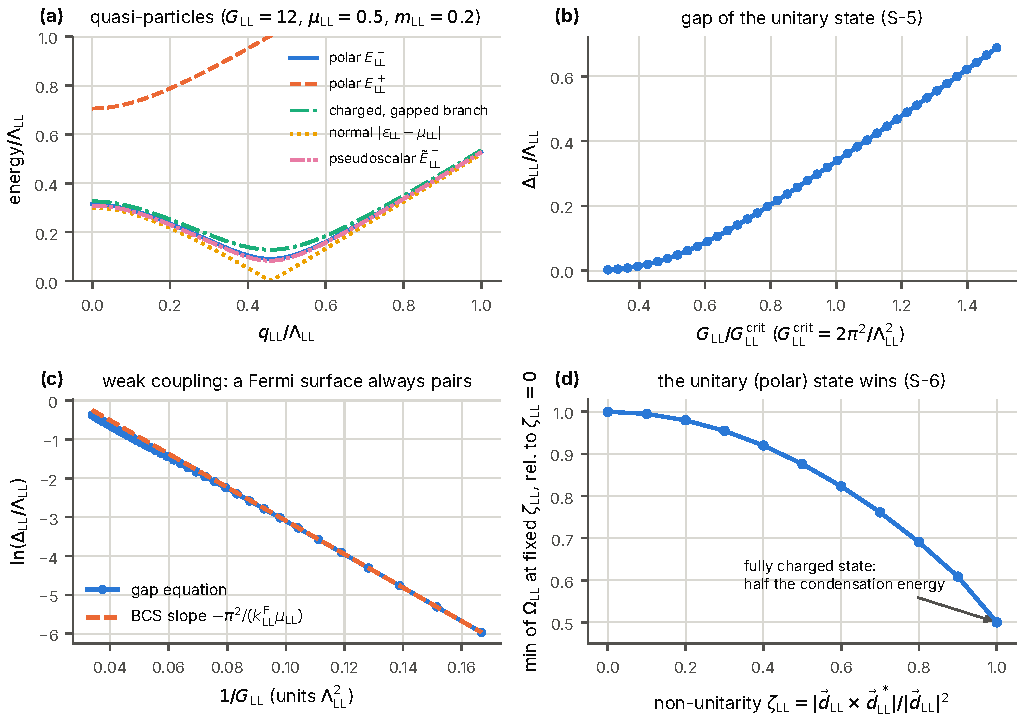
\includegraphics[width=\textwidth]{../figures/fig_sl_superfluid.pdf}
\caption{The spin-zero superfluid of the spinor charges ($\Lambda_{\rm LL}=1$). (a) Quasi-particle
energies versus momentum at $G_{\rm LL}=12$, $\mu_{\rm LL}=0.5$, $m_{\rm LL}=0.2$ (gap
{{GEN:gap_G12}}): the polar state, the gapped branch of the charged state, the normal state and the
pseudoscalar channel at the same gap (Theorem SF2). (b) The gap of the unitary state versus the coupling
in units of $G^{\rm crit}_{\rm LL}$ at $m_{\rm LL}=0$, Eq.~(\ref{eq:gcrit}). (c) Weak coupling: $\ln\Delta_{\rm
LL}$ versus $1/G_{\rm LL}$ and the slope of Bardeen, Cooper and Schrieffer (S-5). (d) The minimum of
$\Omega_{\rm LL}$ at fixed non-unitarity $\zeta_{\rm LL}$, relative to the unitary state (Theorem SF3).}
\label{fig:superfluid}
\end{figure*}
